\documentclass[10pt, conference]{IEEEtran}
\IEEEoverridecommandlockouts

\usepackage{cite}
\usepackage{amsmath,amssymb,amsfonts}
\usepackage{algorithmic}
\usepackage{graphicx}
\usepackage{textcomp}
\usepackage{xcolor}
\usepackage{setspace}
\usepackage{hyperref}
\usepackage{booktabs}
\usepackage{multirow}
\usepackage{mathptmx} % Para usar Times New Roman
\usepackage[utf8]{inputenc} % Para caracteres en español
\usepackage[spanish]{babel} % Para ajustar al idioma español

\def\BibTeX{{\rm B\kern-.05em{\sc i\kern-.025em b}\kern-.08em
    T\kern-.1667em\lower.7ex\hbox{E}\kern-.125emX}}

\begin{document}
\onehalfspacing % Establece el interlineado a 1.5

\title{Procesamiento Digital de Señales ECG Fetales No Invasivas para la Detección de Arritmias}

\author{
	\IEEEauthorblockN{Maximiliano Gaete Pizarro}
	\IEEEauthorblockA{
		Estudiante de Ingeniería Civil Biomédica\\
		\textit{Departamento de Ingeniería Biomédica} \\
		\textit{Universidad de Valparaíso}\\
		Valparaíso, Chile \\
		maximiliano.gaete@alumnos.uv.cl}
	\and
	\IEEEauthorblockN{David Ortiz Puerta}
	\IEEEauthorblockA{
		Doctorado en Cs. de la Ingeniería Civil (PUC)\\
		\textit{Departamento de Ingeniería Biomédica} \\
		\textit{Universidad de Valparaíso}\\
		Valparaíso, Chile \\
		david.ortiz@uv.cl}
}

\maketitle

\begin{abstract}

El electrocardiograma fetal no invasivo permite monitorear la salud del feto mediante señales recogidas en el abdomen materno, ofreciendo una alternativa segura y sin riesgos frente a los métodos invasivos. Se tiene como objetivo desarrollar técnicas de procesamiento digital de señales para mejorar la detección de arritmias fetales en registros ECG no invasivos. Utilizando la base de datos Non-Invasive Fetal ECG Arrhythmia Database (NIFEA DB).
Las señales fueron normalizadas y contaminadas intencionalmente con ruido eléctrico. Se aplicaron filtros pasa-bajas y pasa-altas de Butterworth, filtros FIR y técnicas de filtrado en el dominio de la frecuencia mediante FFT y Zero Padding. Se evaluó la calidad de las señales procesadas mediante la relación señal-ruido (SNR) y el error cuadrático medio (MSE).
Los resultados demuestran que estos filtros efectivamente son eficaces en eliminar las señales contaminantes y en la precisión de la detección de arritmias en señales con ruido, destacando la importancia de estos métodos para un diagnóstico prenatal más confiable. Este avance es crucial en el ámbito biomédico, ya que facilita la identificación temprana de condiciones cardiacas críticas, contribuyendo al bienestar fetal y neonatal.

\end{abstract}

\section{Introducción}

El electrocardiograma (ECG) fetal no invasivo es esencial para monitorear el bienestar fetal durante el embarazo, pues permite obtener la señal cardíaca del feto a través de electrodos en la superficie abdominal materna. Este enfoque evita procedimientos invasivos que podrían comprometer la salud materna o fetal. No obstante, la señal suele verse afectada por ruido eléctrico, interferencias del ECG materno y otros artefactos, lo que dificulta su análisis y diagnóstico.

\begin{figure}[htbp]
	\centerline{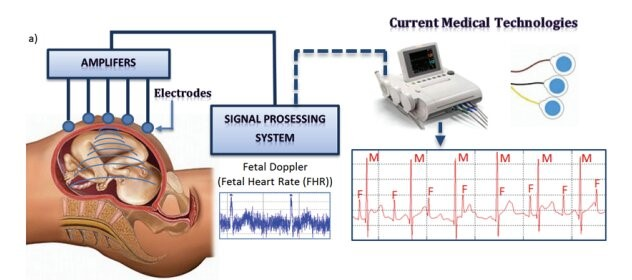
\includegraphics[width=0.5\textwidth]{The-fetal-ECG-monitoring-a-Non-invasive.jpg}}
	\caption{Ejemplo de obtención de señal ECG fetal no invasiva \cite{sensors2022}.}
	\label{fig:fetal_ecg}
\end{figure}

Uno de los mayores desafíos es la detección de arritmias fetales, entendidas como alteraciones del ritmo cardíaco cuya frecuencia excede los rangos considerados normales. Aunque muchas son benignas, algunas requieren atención inmediata. La complejidad radica en la baja amplitud de la señal fetal y en la presencia de ruido y artefactos que dificultan la identificación de patrones característicos.

Ante esta problemática, resulta necesario aplicar técnicas de procesamiento digital de señales para mejorar la separación de la señal fetal y optimizar la detección de arritmias. En este estudio se emplearon datos de la base \textit{Non-Invasive Fetal ECG Arrhythmia Database (NIFEA DB)} \cite{behar2019noninvasive}, aplicando estrategias de preprocesamiento y filtrado.

\subsection{Descripción del Estudio}

El objetivo principal es desarrollar y aplicar métodos de procesamiento de señales que mejoren la detección de arritmias en ECG fetales no invasivos. Se parte de la hipótesis de que, mediante filtrados y análisis adecuados, es posible extraer la señal fetal y reconocer patrones de arritmia. Esta iniciativa tiene un potencial impacto clínico, pues contribuiría al diagnóstico temprano y al tratamiento oportuno de problemas cardíacos fetales.

\subsection{Equipos, Metodología de Procesamiento y Ruidos de la Señal}

Los registros se obtuvieron con electrodos de superficie en abdomen y pecho maternos, incluyendo múltiples canales abdominales y uno torácico, con frecuencias de muestreo de 500 Hz o 1 kHz.

Entre las fuentes de ruido se identifican:
\begin{itemize}
	\item \textbf{Señal ECG Materna (MECG):} Puede enmascarar los complejos QRS fetales debido a su mayor amplitud.
	\item \textbf{Ruido Muscular (EMG):} Generado por la actividad de músculos uterinos y abdominales.
	\item \textbf{Interferencias Electromagnéticas:} Provenientes de la línea eléctrica y el entorno.
	\item \textbf{Movimiento Materno y Fetal:} Cambios en la impedancia y artefactos por movimientos involuntarios.
\end{itemize}

La combinación de estos ruidos requiere el uso de filtrado adaptativo, análisis de componentes independientes y algoritmos especializados en supresión de artefactos.

\subsection{Fisiología de la Señal y Umbrales de Variables}

La señal ECG fetal refleja la actividad eléctrica del corazón. Su frecuencia cardíaca normal oscila entre 110 y 160 bpm; valores fuera de este rango pueden indicar bradicardia o taquicardia. Asimismo, la amplitud de la señal fetal suele encontrarse entre 10 µV y 50 µV, lo que dificulta su distinción respecto de la señal materna. Los intervalos temporales y la morfología de los complejos QRS permiten identificar arritmias como extrasístoles, taquicardias supraventriculares o bloqueos auriculoventriculares.

\begin{figure}[htbp]
	\centerline{\includegraphics[width=0.5\textwidth]{Señal-sana completa.png}}
	\caption{Señal ECG fetal completa.}
	\label{fig:complete_signal}
\end{figure}

\subsection{Población de Estudio y Condiciones de Adquisición}

La población de estudio incluye fetos con diagnóstico de arritmia (ARR) y con ritmo cardíaco normal (NR), registrados en entornos clínicos controlados, preferentemente en el tercer trimestre de gestación. Aunque se busca minimizar factores externos, la posición fetal, el índice de masa corporal materno y los movimientos involuntarios pueden añadir variabilidad y ruido a las señales.
\section{Objetivos}

\subsection{Objetivo General}

Desarrollar técnicas de procesamiento digital para señales ECG fetales no invasivas que permitan la identificación de arritmias en señal con ruido con el propósito de demostrar que estas técnicas son efectivas.

\subsection{Objetivos Específicos}

Para alcanzar este propósito, inicialmente se busca aplicar estrategias de preprocesamiento y filtrado que mejoren la relación señal-ruido, favoreciendo una detección más confiable de la actividad fetal. Una vez obtenidas señales más limpias, se pretende identificar y extraer características clave que evidencien la presencia de arritmias, facilitando su diagnóstico temprano. Finalmente, se llevarán a cabo análisis espectrales y temporales a fin de evaluar la información contenida en las señales procesadas y contrastar sus resultados con registros normales, estableciendo así referencias que orienten la toma de decisiones clínicas.

\section{Estado del arte}

La detección de arritmias fetales a través del electrocardiograma (ECG) no invasivo es un área de investigación activa debido a su potencial para mejorar el monitoreo prenatal y la detección temprana de anomalías cardíacas~\cite{behar2014non}. La obtención de la señal ECG fetal a partir de electrodos colocados en el abdomen materno presenta desafíos significativos debido a la baja amplitud de la señal fetal y a la presencia de ruido e interferencias, principalmente del ECG materno y de otros artefactos fisiológicos y ambientales~\cite{martens2007robust}.

Diversas técnicas de procesamiento de señales han sido desarrolladas para extraer eficazmente la señal ECG fetal. Entre ellas, el Análisis de Componentes Independientes (ICA, por sus siglas en inglés) ha sido ampliamente utilizado para separar las señales fetal y materna basándose en la independencia estadística de las fuentes~\cite{delathauwer2000fetal, zarzoso2001noninvasive}. Por ejemplo, De Lathauwer \textit{et al.} aplicaron ICA para separar las señales, obteniendo resultados prometedores en la extracción del ECG fetal~\cite{delathauwer2000fetal}.

Otra técnica común es el uso de filtros adaptativos, donde el ECG materno registrado en el tórax se utiliza como referencia para eliminar su contribución en los registros abdominales~\cite{widrow1975adaptive}. Sameni \textit{et al.} propusieron un método basado en modelos dinámicos y filtrado de Kalman para mejorar la calidad de la señal fetal extraída~\cite{sameni2008nonlinear}.

Además, los métodos basados en transformadas wavelet han demostrado ser efectivos en la detección de los complejos QRS fetales debido a su capacidad para analizar señales no estacionarias~\cite{addison2005wavelet}. Kotas utilizó la Transformada Wavelet Discreta para mejorar la detección de eventos cardíacos fetales en presencia de ruido~\cite{kotas2007detection}.

En cuanto a la detección de arritmias, algunas investigaciones se han centrado en el análisis de intervalos RR y la identificación de patrones irregulares en la frecuencia cardíaca fetal~\cite{taylor2003fetal}. Xu \textit{et al.} desarrollaron un algoritmo para la detección automática de arritmias utilizando técnicas de aprendizaje automático sobre señales ECG fetales no invasivas~\cite{xu2004rpeak}.

Las bases de datos disponibles públicamente, como la \textit{Non-Invasive Fetal ECG Arrhythmia Database} (NIFEA DB)\cite{behar2014non} y las bases de datos del \textit{PhysioNet/Computing in Cardiology Challenge}\cite{clifford2013physionet}, han sido fundamentales para el desarrollo y validación de estos métodos. Estas bases de datos proporcionan registros reales con anotaciones que permiten evaluar el desempeño de los algoritmos propuestos.

A pesar de los avances, persisten desafíos en la detección precisa de arritmias fetales debido a la variabilidad interindividual, la baja relación señal-ruido y la necesidad de métodos robustos que puedan aplicarse en tiempo real en entornos clínicos~\cite{andreotti2018clinical}. Por lo tanto, la investigación continúa enfocándose en el desarrollo de técnicas más avanzadas de procesamiento de señales y aprendizaje automático para mejorar la exactitud y confiabilidad de la detección de arritmias fetales.

\section{Técnicas de Procesamiento}


Se llevó a cabo diversas técnicas de procesamiento digital aplicadas a las señales ECG fetales no invasivas, con el objetivo de mejorar la detección de arritmias en presencia de ruido. Las etapas de procesamiento incluyen el preprocesamiento de las señales, el análisis espectral y temporal, la contaminación intencional de las señales con ruido blanco gaussiano y artefactos de movimiento para evaluar y simular ruido real en las mediciones puras para las técnicas de filtrado, y otros análisis complementarios para extraer características relevantes.

\subsection{Preprocesamiento de la Señal}

Para realizar un preprocesamiento adecuado de la señal, es fundamental comprender cómo influye este paso en su análisis posterior. En este contexto, la normalización de la señal se lleva a cabo utilizando la siguiente ecuación:

\[
s'(n) = \frac{s(n)}{\max(|s(n)|)}
\]

Este proceso garantiza que la señal esté escalada al rango \([-1, 1]\), facilitando la comparación entre señales y mejorando la estabilidad numérica.

Se identificó que las señales tienen una frecuencia de muestreo de \( f_s = 1000 \, \text{Hz} \), lo cual es adecuado para captar la actividad cardíaca fetal. El número de muestras y el intervalo de Nyquist se calcularon de la siguiente manera:

\begin{itemize}
    \item \textbf{Frecuencia de muestreo:} \( f_s = 1000 \, \text{Hz} \)
    \item \textbf{Número de muestras:} \( N = 5000 \)
    \item \textbf{Intervalo de Nyquist:} 
    \[
    f_N = \frac{f_s}{2} = 500 \, \text{Hz}
    \]
\end{itemize}

Para el análisis, se seleccionó un segmento específico de las señales, enfocándose en intervalos donde se presentan arritmias o eventos de interés. Esto permite analizar únicamente la porción relevante de la señal, mejorando la eficiencia del procesamiento y reduciendo la carga computacional.

El intervalo temporal de interés seleccionado comprende las muestras entre los índices \( n_1 = 1200 \) y \( n_2 = 6200 \), lo que corresponde a la porción:

\[
\text{Señal de interés: } s'(n) = s(n), \quad \forall n \in [1200, 6200]
\]

Donde \( s'(n) \) representa el segmento de la señal utilizado para el análisis y \( s(n) \) la señal original.

Con el fin de evaluar la eficacia de los métodos de filtrado, se contaminó intencionalmente la señal original con ruido que representa condiciones reales de adquisición. Los tipos de ruido añadidos fueron los siguientes:

\begin{figure}[htbp]
	\centerline{\includegraphics[width=0.5\textwidth]{Señal-vetana.png}}
	\caption{Comparación del canal 2 con y sin presencia de una arritmia.}
	\label{fig:ecg_sano}
\end{figure}

\subsubsection{Ruido eléctrico (50 Hz)}
Se simuló la interferencia de la red eléctrica, común en entornos de adquisición. Este ruido se generó utilizando una onda sinusoidal con frecuencia de \( 50 \, \text{Hz} \) y se modeló de la siguiente forma:

\[
r_{\text{eléctrico}}(t) = A \cdot \sin(2 \pi f t)
\]

\subsubsection{Ruido muscular (EMG)}
Se simuló la actividad eléctrica de los músculos uterinos y abdominales como ruido de tipo aleatorio con distribución normal, modelado de la siguiente manera:

\[
r_{\text{EMG}}(n) = A \cdot \mathcal{N}(0, 1)
\]

\subsubsection{Señal contaminada}
La señal contaminada se obtuvo sumando los dos tipos de ruido a la señal original:

\[
s_{\text{contaminada}}(n) = s(n) + r_{\text{eléctrico}}(n) + r_{\text{EMG}}(n)
\]

\begin{figure}[htbp]
	\centerline{\includegraphics[width=0.5\textwidth]{Señal-con ruido.png}}
	\caption{Señal ECG fetal contaminada con ruido eléctrico y muscular.}
	\label{fig:signal_with_noise}
\end{figure}


\subsection{Procesamiento de la Señal}

Se realizó el análisis espectral de las señales utilizando la Transformada de Fourier (FFT). La señal se representó en decibeles para visualizar las componentes frecuenciales, según la siguiente expresión:

\[
X(f) = \mathcal{F}\{x(t)\} = \int_{-\infty}^{\infty} x(t) e^{-j 2 \pi f t} dt
\]

Este análisis permitió identificar las principales frecuencias presentes en las señales y ajustar los filtros en consecuencia.

\begin{figure}[htbp]
\centerline{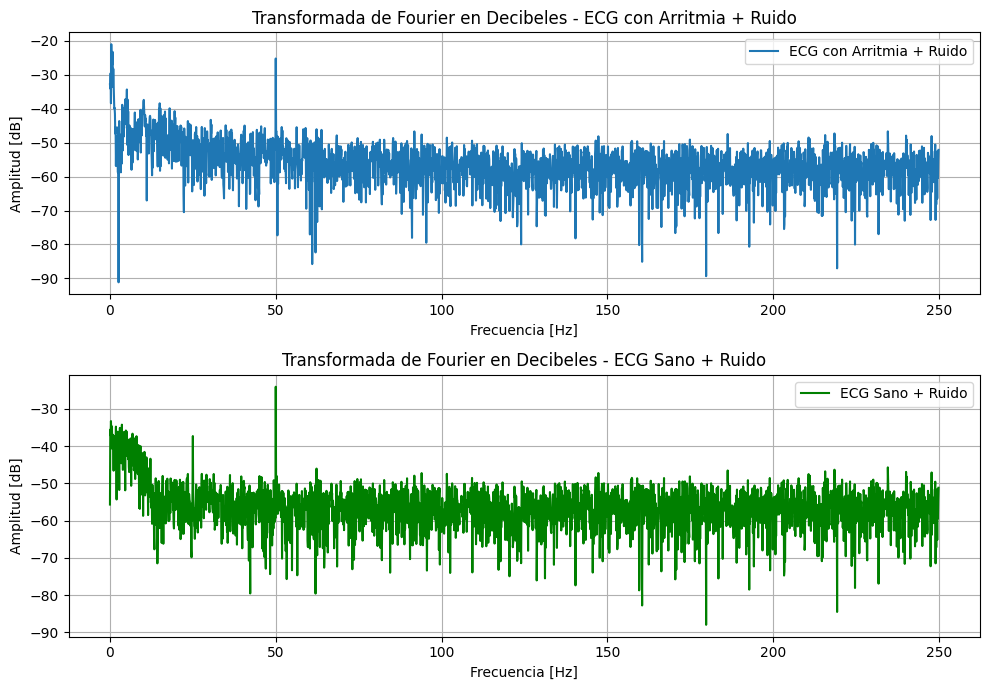
\includegraphics[width=0.5\textwidth]{ftt.png}}
\caption{Transformada de Fourier de la señal ECG fetal.}
\label{fig:fft_signal}
\end{figure}

\subsubsection{Espectrogramas}
Se generaron espectrogramas para visualizar cómo las frecuencias de la señal varían en el tiempo. Utilizando ventanas de tipo Hann y solapamiento del 75\%, se aplicó la Transformada de Fourier de corto tiempo (STFT), definida como:

\[
S(t, f) = \int_{-\infty}^{\infty} x(\tau) w(\tau - t) e^{-j 2 \pi f \tau} d\tau
\]

\begin{figure}[htbp]
	\centerline{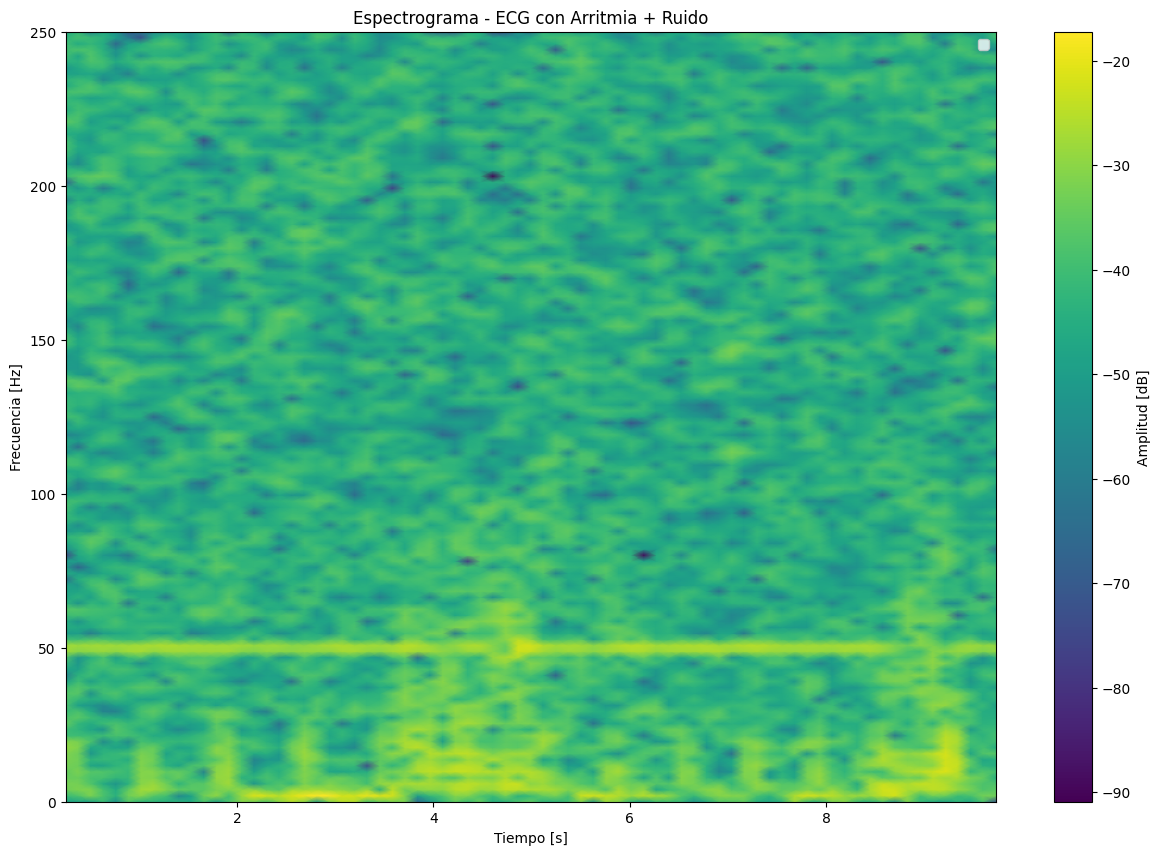
\includegraphics[width=0.5\textwidth]{Espectrograma - ECG con Arritmia + Ruido.png}}
	\caption{Espectrograma de la señal ECG fetal con arritmia.}
	\label{fig:espectrograma_con_arritmia}
	\end{figure}

\begin{figure}[htbp]
	\centerline{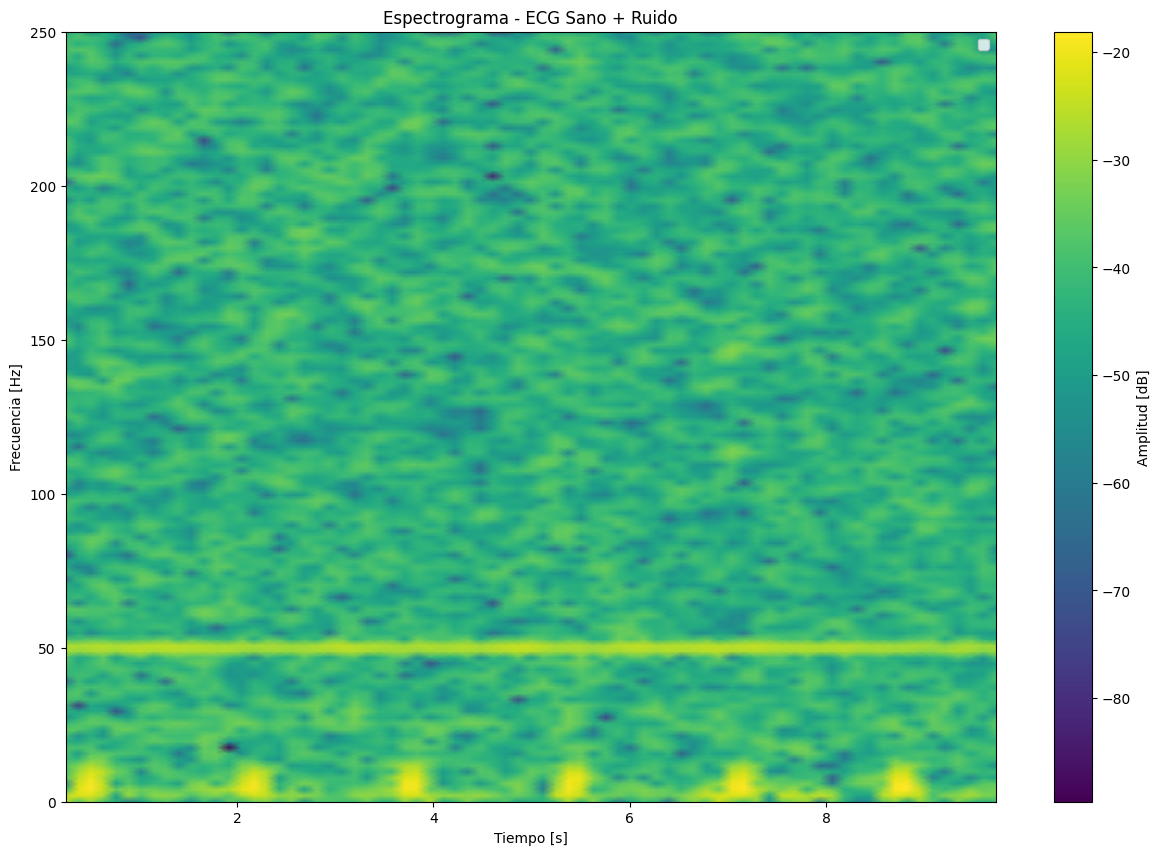
\includegraphics[width=0.5\textwidth]{Espectrograma ECG Sano + Ruido.png}}
	\caption{Espectrograma de la señal ECG fetal sin arritmia.}
	\label{fig:espectrograma_sin_arritmia}
\end{figure}

\subsubsection{Filtros Pasa-Bajas y Pasa-Altas}

Para eliminar el ruido de alta frecuencia y las componentes de baja frecuencia no deseadas, se diseñaron filtros pasa-bajas y pasa-altas. Las frecuencias de corte seleccionadas despues del analisis fueron:

\begin{itemize}
	\item \textbf{Frecuencia de corte pasa-bajas:} \( f_{\text{corte\_bajas}} = 50 \, \text{Hz} \)
	\item \textbf{Frecuencia de corte pasa-altas:} \( f_{\text{corte\_altas}} = 0.5 \, \text{Hz} \)
\end{itemize}


\subsubsection{Detección de picos en la señal}
Para analizar el ritmo cardíaco fetal y detectar posibles arritmias, se implementó la detección de picos. Se asumió un rango de frecuencia cardíaca fetal entre 120 y 160 latidos por minuto (bpm), correspondiente a un intervalo RR mínimo de:

\[
T_{\text{RR\_mín}} = \frac{60}{160} = 0.375 \, \text{s}
\]

La detección se realizó buscando máximos locales con una distancia mínima entre picos de \( d = T_{\text{RR\_mín}} \cdot f_s \).

\begin{figure}[htbp]
	\centerline{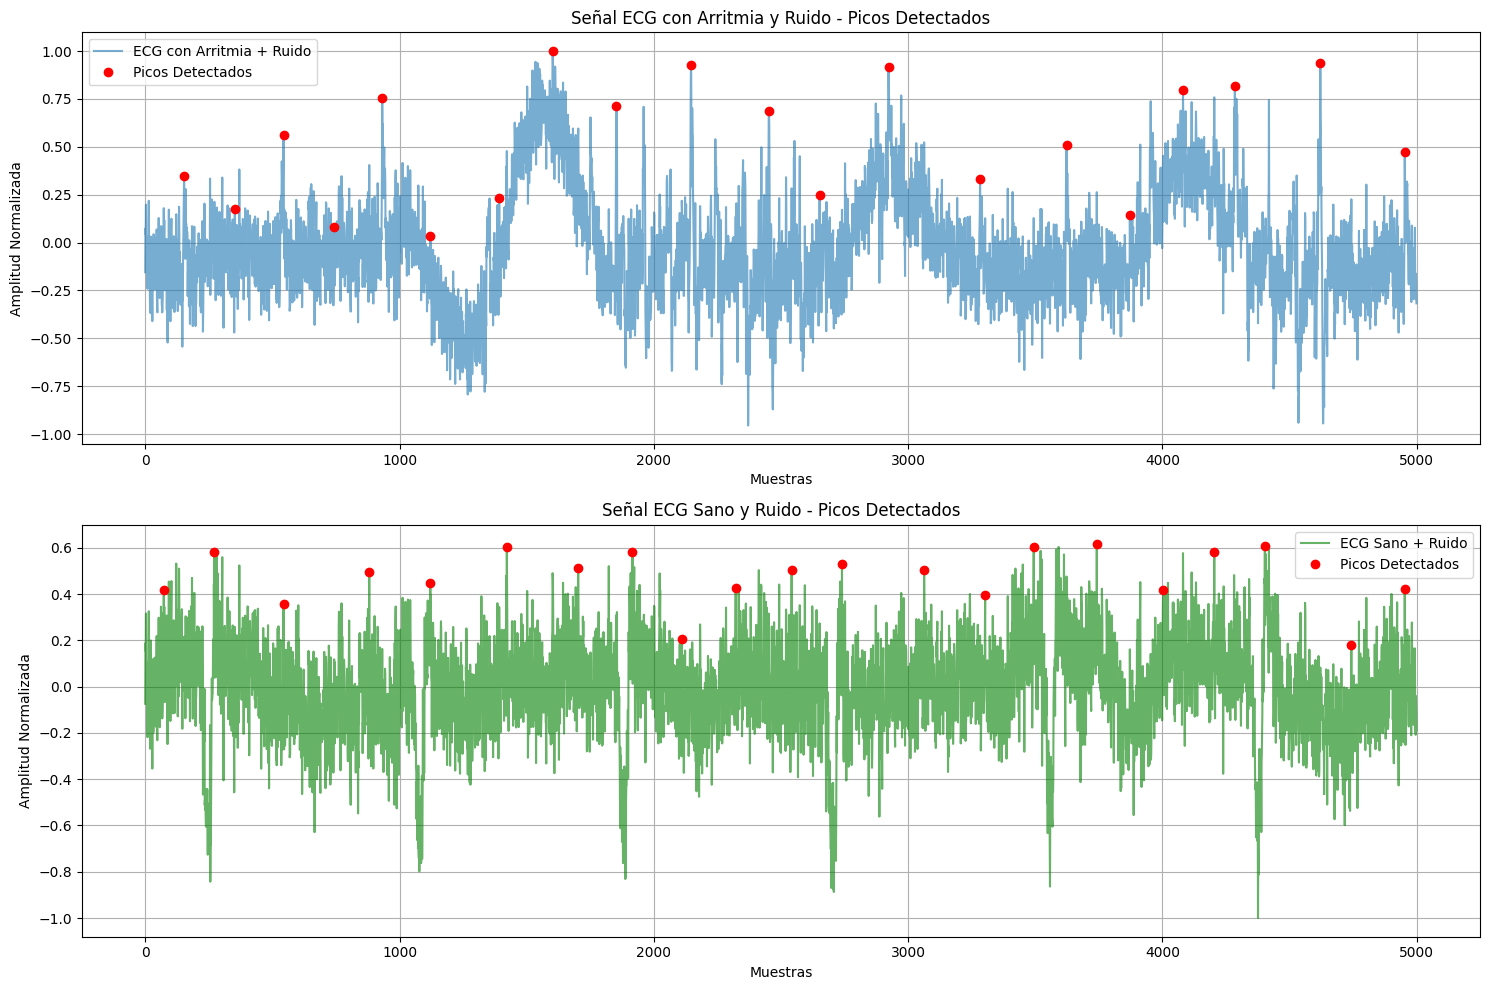
\includegraphics[width=0.45\textwidth]{picos.png}}
	\caption{Detección de picos en la señal ECG fetal.}
	\label{fig:peak_detection}
\end{figure}

\subsection{Diseño e implementación de técnicas de filtrado}

Para evaluar la calidad de la señal, se calcularon el SNR (\textit{Signal-to-Noise Ratio}) y el MSE (\textit{Mean Squared Error}) entre la señal original y la señal contaminada. Las expresiones utilizadas fueron:

Relación señal-ruido (SNR):
    \[
    \text{SNR} = 10 \cdot \log_{10}\left(\frac{P_{\text{señal}}}{P_{\text{ruido}}}\right)
    \]

Error cuadrático medio (MSE):
    \[
    \text{MSE} = \frac{1}{N} \sum_{n=1}^N \left[s(n) - y(n)\right]^2
    \]

El SNR fue calculado antes del filtrado fue:

Resultados antes del filtrado para la Señal con Arritmia:
	\begin{itemize}
		\item SNR antes del filtrado: -5.03 dB
		\item MSE antes del filtrado: 0.038727
	\end{itemize}

Resultados antes del filtrado para la Señal Sana:
	\begin{itemize}
		\item SNR antes del filtrado: -11.96 dB
		\item MSE antes del filtrado: 0.052139
	\end{itemize}

\subsubsection{Implementación}
Se implementaron diversas técnicas de filtrado para eliminar el ruido de las señales contaminadas:

\paragraph{Filtros IIR (Butterworth)}
Se diseñaron filtros pasa-bajas y pasa-altas de tipo Butterworth, caracterizados por una respuesta en frecuencia suave y sin ondulaciones. La función de transferencia se define como:

\[
H(s) = \frac{1}{1 + \left(\frac{s}{\omega_c}\right)^{2n}}
\]

\paragraph{Filtros FIR}
Se diseñaron filtros FIR utilizando ventanas de Hamming. La respuesta al impulso del filtro se calculó como:

\[
h[n] = w[n] \cdot \text{sinc}\left(\frac{2f_c}{f_s}(n - M/2)\right)
\]


\paragraph{Filtrado mediante FFT y Zero Padding}
El filtrado en el dominio de la frecuencia se realizó aplicando una Transformada de Fourier (FFT) y creando una máscara de paso banda. La señal filtrada se obtuvo como:

\[
Y(f) = X(f) \cdot H(f)
\]

\subsection{Comparación y evaluación de los filtros}

Para ilustrar de manera clara el desempeño de las diferentes técnicas de filtrado aplicadas, se presentarán los gráficos correspondientes a los resultados obtenidos después de cada proceso de filtrado.

A través de estas representaciones gráficas, será posible observar cómo cada filtro afecta la señal y evaluar visualmente su eficacia en términos de eliminación de ruido y conservación de las amplitudes originales. Esta comparación facilitará la identificación de la técnica más adecuada para el procesamiento de señales ECG fetales, en función de la calidad de la señal reconstruida.

\begin{figure}[htbp]
\centerline{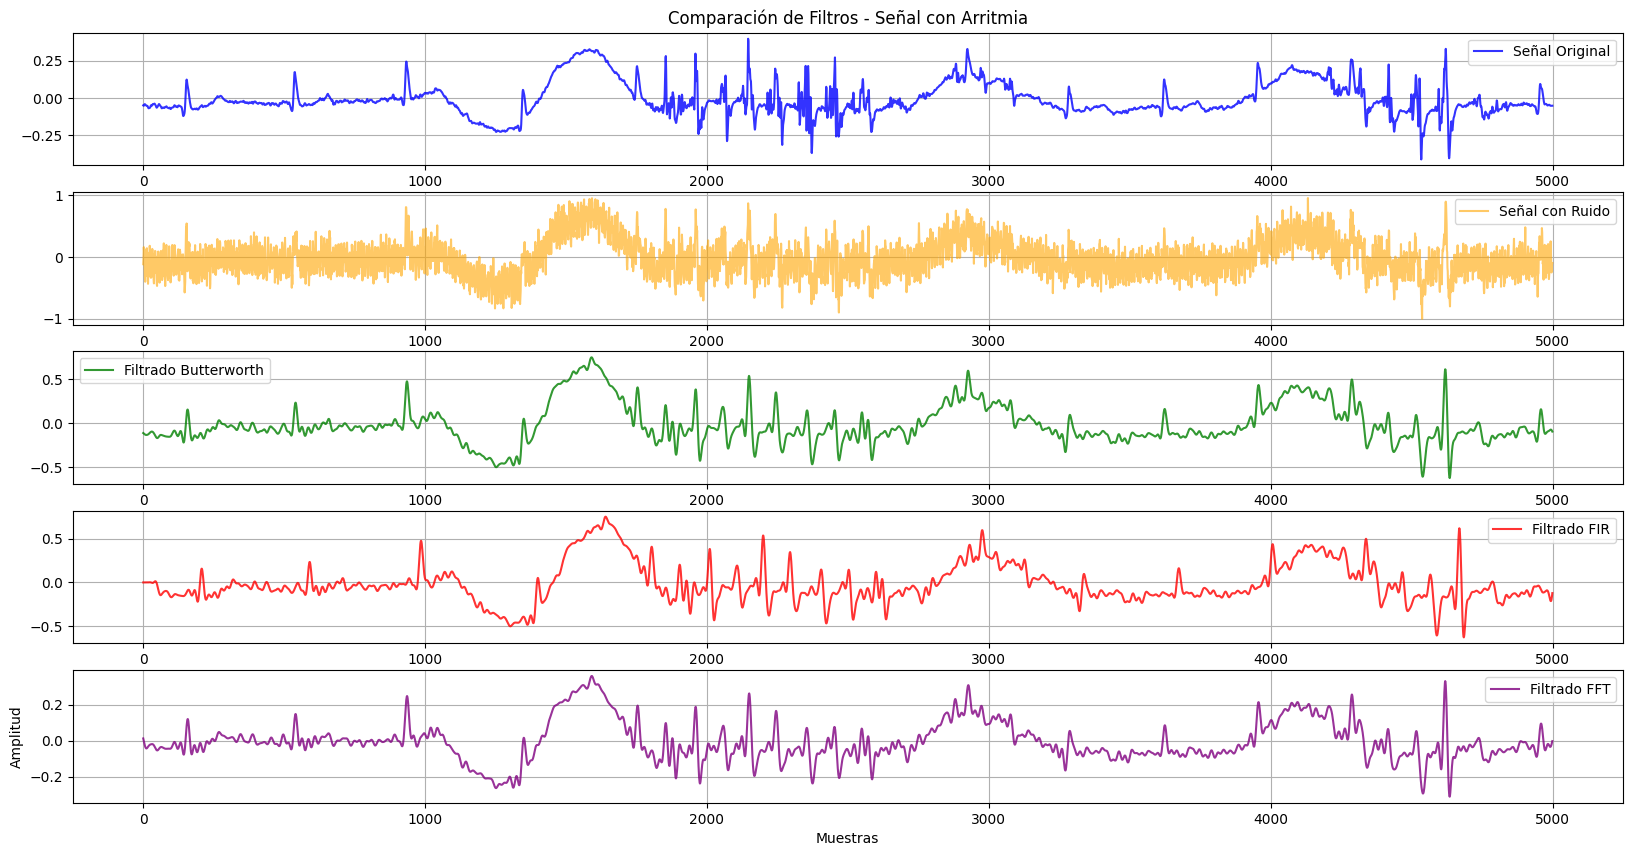
\includegraphics[width=0.5\textwidth]{Comparacion arritmia.png}}
\caption{Comparacion de tecnicas de filtrado señal ECG con presencia de arritmia.}
\label{fig:filtered_signal}
\end{figure}

\begin{figure}[htbp]
\centerline{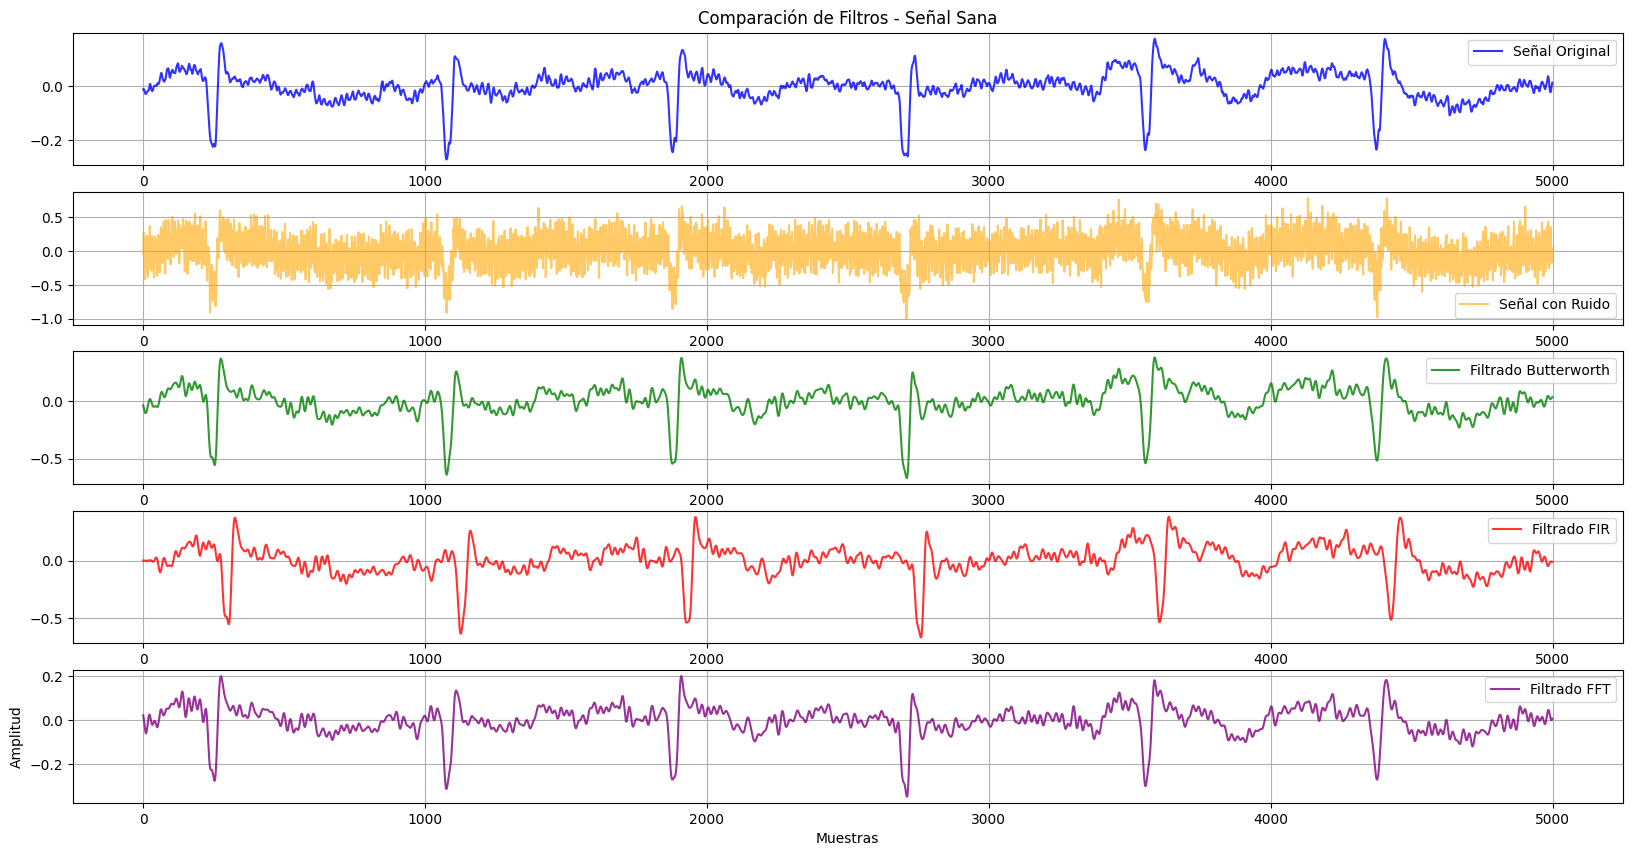
\includegraphics[width=0.5\textwidth]{Comparacion normal.png}}
\caption{Comparacion de tecnicas de filtrado señal ECG normal.}
\label{fig:comparison_signal}
\end{figure}

El SNR y el MSE se calcularon para cada técnica de filtrado, comparando los resultados obtenidos con las señales contaminadas y las señales originales. Estos valores permitieron evaluar la eficacia de los filtros en la eliminación del ruido y la mejora de la calidad de la señal.

\begin{table}[h!]
	\centering
	\caption{Comparación de SNR y MSE antes y después del filtrado}
	\label{tab:snr_mse_comparison}
	\begin{tabular}{l l c c}
	\toprule
	\textbf{Señal} & \textbf{Condición} & \textbf{SNR (dB)} & \textbf{MSE} \\
	\midrule
	\multirow{2}{*}{\textbf{Arritmica}} & Antes & -5.76 & 0.045812 \\
	 & Butterworth & -0.59 & 0.013952 \\
	 & FIR & -3.76 & 0.028924 \\
	 & FFT Zero Padding & 10.09 & 0.001193 \\
	\midrule
	\multirow{2}{*}{\textbf{Sana}} & Antes & -11.48 & 0.046723 \\
	 & Butterworth & -2.89 & 0.006459 \\
	 & FIR & -7.56 & 0.018936 \\
	 & FFT Zero Padding & 8.23 & 0.000499 \\
	\bottomrule
	\end{tabular}
\end{table}

\subsection{Analisis de la Señal Procesada}

Después de emplear las métricas cuantitativas, como la relación señal-ruido (SNR) y el error cuadrático medio (MSE), así como representaciones gráficas que ilustran visualmente el efecto de cada técnica sobre las características de la señal original, los resultados permiten identificar la técnica más adecuada para el procesamiento de señales ECG fetales, priorizando la eliminación efectiva del ruido y la conservación de las amplitudes originales \cite{sensors2022}, \cite{behar2019noninvasive}. 

En el caso de las señales con arritmia, se observó una mejora significativa con la técnica de FFT Zero Padding, que incrementó el SNR de -5.76 dB a 10.09 dB, representando un aumento del 275 \% respecto al SNR inicial. Asimismo, el MSE se redujo de 0.045812 a 0.001193, lo que equivale a una mejora del 97.4 \% en el error cuadrático medio. Comparativamente, el filtro Butterworth mejoró el SNR en un 89.7 \%, alcanzando -0.59 dB, mientras que el MSE disminuyó un 69.5 \%. 

El filtro FIR, aunque menos efectivo, logró mejoras del 34.7 \% en el SNR y del 36.9 \% en el MSE. Para las señales normales, los resultados muestran que la técnica FFT Zero Padding incrementó el SNR de -11.48 dB a 8.23 dB, con un aumento del 171.7 \%, y redujo el MSE en un 98.9 \%, de 0.046723 a 0.000499. Por otro lado, el filtro Butterworth logró un incremento del SNR del 74.8 \% y una reducción del MSE del 86.2 \%, mientras que el filtro FIR mejoró el SNR en un 34.2 \% y el MSE en un 59.5 \%.

\section{Conclusión}

El electrocardiograma (ECG) fetal no invasivo representa una herramienta clave en la monitorización del bienestar fetal, brindando una alternativa segura y eficaz para evaluar la actividad eléctrica del corazón fetal sin recurrir a procedimientos invasivos. Sin embargo, este enfoque enfrenta retos técnicos considerables debido a la presencia de ruido ambiental, interferencias del ECG materno y artefactos asociados al movimiento, los cuales complican la extracción y análisis de la señal fetal \cite{addison2005wavelet}. 

La detección temprana de arritmias fetales mediante estas técnicas es crítica para prevenir complicaciones severas y garantizar una intervención oportuna \cite{kotas2007detection}. El presente estudio refuerza la importancia de optimizar las etapas de preprocesamiento y análisis espectral para mejorar la calidad de las señales ECG fetales \cite{taylor2003fetal}. Asimismo, el diseño de filtros adaptados y técnicas de detección de picos permite una evaluación más precisa de las arritmias, contribuyendo al diagnóstico y manejo clínico en tiempo real \cite{xu2004rpeak}. Los resultados obtenidos, medidos en términos de mejora del SNR y reducción del MSE, validan la efectividad de las estrategias implementadas y subrayan su potencial en aplicaciones clínicas \cite{clifford2013physionet}. 

La técnica de FFT Zero Padding se consolida como la más efectiva para el procesamiento de señales ECG, dado que ofrece mejoras significativamente superiores tanto en SNR como en MSE en comparación con los métodos Butterworth y FIR. Estas mejoras reflejan una capacidad sobresaliente para eliminar ruido, preservar la morfología de la señal y garantizar que las amplitudes originales se mantengan intactas. Este rendimiento hace que FFT Zero Padding sea la técnica ideal para aplicaciones clínicas y diagnósticas que dependen de señales ECG precisas. En el ámbito biomédico, la calidad de las señales procesadas es crucial para garantizar diagnósticos fiables. Una señal ECG limpia permite identificar con precisión los picos en cada ciclo del ECG, así como los intervalos entre ellos, que son fundamentales para diagnosticar y clasificar arritmias. 

La presencia de ruido puede enmascarar estas características, llevando a interpretaciones erróneas y posibles errores diagnósticos. Por tanto, el desarrollo de técnicas de filtrado eficientes no solo mejora la interpretación clínica, sino que también contribuye a la implementación de sistemas automatizados de monitoreo, aumentando la seguridad y la eficacia del diagnóstico médico \cite{de2014efficient}. La capacidad de identificar de manera precisa irregularidades en el ritmo cardíaco asegura intervenciones tempranas y reduce los riesgos asociados a enfermedades cardíacas no detectadas \cite{behar2014non}.

\begin{thebibliography}{00}

	\bibitem{sensors2022} S. F. Abdul Halim, Z. Zakaria, J. Pusppanathan, A. Mohd Noor, A. N. Norali, M. H. Fazalul Rahiman, S. Z. Mohd Muji, R. Abdul Rahim, E. I. Engku-Husna, M. K. Ali Hassan et al., “A review on magnetic induction spectroscopy potential for fetal acidosis examination,” Sensors, vol. 22, no. 4, p. 1334, 2022.

	\bibitem{behar2019noninvasive} J. A. Behar, L. Bonnemains, V. Shulgin, J. Oster, O. Ostras, and I. Lakhno, ``Noninvasive fetal electrocardiography for the detection of fetal arrhythmias,'' \textit{Prenatal Diagnosis}, vol. 39, no. 3, pp. 178--187, 2019.

	\bibitem{goldberger2000physiobank} A. L. Goldberger \textit{et al.}, ``PhysioBank, PhysioToolkit, and PhysioNet: components of a new research resource for complex physiologic signals,'' \textit{Circulation}, vol. 101, no. 23, pp. e215--e220, 2000.

	\bibitem{de2014efficient} S. De, K. Dandapat, and P. K. Dutta, ``Efficient fetal ECG extraction from abdominal ECG using narrow band adaptive filtering,'' \textit{Signal, Image and Video Processing}, vol. 8, no. 1, pp. 111--119, 2014.

	\bibitem{behar2014non} J.Behar \emph{etal.}, ``Non-invasive fetal ECG technologies: a review,'' \emph{Pediatric Cardiology}, vol.~35, no.~7, pp. 1083--1092, 2014.

	\bibitem{martens2007robust} S.M. Martens \emph{etal.}, ``A robust fetal ECG detection method for abdominal recordings,'' \emph{Physiological Measurement}, vol.~28, no.~4, p. 373, 2007.

	\bibitem{delathauwer2000fetal} L.DeLathauwer, B.DeMoor, and J.~Vandewalle, ``Fetal electrocardiogram extraction by blind source subspace separation,'' \emph{IEEE Transactions on Biomedical Engineering}, vol.~47, no.~5, pp. 567--572, 2000.

	\bibitem{zarzoso2001noninvasive} V.~Zarzoso and A.~K. Nandi, ``Noninvasive fetal electrocardiogram extraction: Blind separation versus adaptive noise cancellation,'' \emph{IEEE Transactions on Biomedical Engineering}, vol.~48, no.~1, pp. 12--18, 2001.

	\bibitem{widrow1975adaptive} B.Widrow \emph{etal.}, ``Adaptive noise cancelling: Principles and applications,'' \emph{Proceedings of the IEEE}, vol.~63, no.~12, pp. 1692--1716, 1975.

	\bibitem{sameni2008nonlinear} R.Sameni \emph{etal.}, ``A nonlinear Bayesian filtering framework for ECG denoising,'' \emph{IEEE Transactions on Biomedical Engineering}, vol.~55, no.~9, pp. 2168--2176, 2008.

	\bibitem{addison2005wavelet} P.~S. Addison, ``Wavelet transforms and the ECG: a review,'' \emph{Physiological Measurement}, vol.~26, no.~5, p. R155, 2005.

	\bibitem{kotas2007detection} M.~Kotas, ``Detection of fetal QRS complexes using the matched filter,'' \emph{Computers in Cardiology}, vol.~34, pp. 85--88, 2007.

	\bibitem{taylor2003fetal} M.~J. Taylor and M.~J. Smith, ``The fetal ECG and fetal arrhythmias,'' \emph{Early Human Development}, vol.~75, pp. S43--S48, 2003.

	\bibitem{xu2004rpeak} S.~Xu, Y.~T. Zhang, and W.~Xu, ``An R-peak detection method for fetal ECG based on joint approximate diagonalization of eigen-matrices,'' \emph{IEEE Transactions on Biomedical Engineering}, vol.~51, no.~6, pp. 1053--1061, 2004.

	\bibitem{clifford2013physionet} G.D. Clifford \emph{etal.}, ``The PhysioNet/computing in cardiology challenge 2013: fetal ECG signal processing,'' \emph{Computing in Cardiology Conference}, vol.~40, pp. 149--152, 2013.

	\bibitem{andreotti2018clinical} F.Andreotti \emph{etal.}, ``Clinical validation of the wearable sensor system for fetal heart rate monitoring,'' \emph{IEEE Transactions on Biomedical Engineering}, vol.~66, no.~3, pp. 810--820, 2018.


\end{thebibliography}

\end{document}